\documentclass[times,specification,annotation]{itmo-student-thesis}
% \linespread{1.4}

%% Опции пакета:
%% - specification - если есть, генерируется задание, иначе не генерируется
%% - annotation - если есть, генерируется аннотация, иначе не генерируется
%% - times - делает все шрифтом Times New Roman, собирается с помощью xelatex
%% - languages={...} - устанавливает перечень используемых языков. По умолчанию это {english,russian}.
%%                     Последний из языков определяет текст основного документа.

%% Делает запятую в формулах более интеллектуальной, например:
%% $1,5x$ будет читаться как полтора икса, а не один запятая пять иксов.
%% Однако если написать $1, 5x$, то все будет как прежде.
\usepackage{icomma}

%% Один из пакетов, позволяющий делать таблицы на всю ширину текста.
\usepackage{tabularx}
\usepackage[unicode=true,implicit=false,hidelinks]{hyperref}

%% Данные пакеты необязательны к использованию в бакалаврских/магистерских
%% Они нужны для иллюстративных целей
%% Начало
\usepackage{tikz}
\usetikzlibrary{arrows}
\usepackage{filecontents}
\begin{filecontents}{bachelor-thesis.bib}
@article{ big-graphs-future-arxiv,
	doi = {10.1145/3434642},
	url = {https://doi.org/10.1145\%2F3434642},
	year = 2021,
	month = {sep},
	publisher = {Association for Computing Machinery ({ACM})},
	volume = {64},
	number = {9},
	pages = {62--71},
	author = {Sherif Sakr and Angela Bonifati and Hannes Voigt and Alexandru Iosup and Khaled Ammar and Renzo Angles and Walid Aref and Marcelo Arenas and Maciej Besta and Peter A. Boncz and Khuzaima Daudjee and Emanuele Della Valle and Stefania Dumbrava and Olaf Hartig and Bernhard Haslhofer and Tim Hegeman and Jan Hidders and Katja Hose and Adriana Iamnitchi and Vasiliki Kalavri and Hugo Kapp and Wim Martens and M. Tamer Özsu and Eric Peukert and Stefan Plantikow and Mohamed Ragab and Matei R. Ripeanu and Semih Salihoglu and Christian Schulz and Petra Selmer and Juan F. Sequeda and Joshua Shinavier and G{\'{a}}bor Sz{\'{a}}rnyas and Riccardo Tommasini and Antonino Tumeo and Alexandru Uta and Ana Lucia Varbanescu and Hsiang-Yun Wu and Nikolay Yakovets and Da Yan and Eiko Yoneki},
	title = {The future is big graphs},
	journal = {Communications of the {ACM}},
	langid = {english}
}

@inproceedings{ gremlin,
    author = {Rodriguez, Marko A.},
    title = {The Gremlin Graph Traversal Machine and Language (Invited Talk)},
    year = {2015},
    isbn = {9781450339025},
    publisher = {Association for Computing Machinery},
    address = {New York, NY, USA},
    url = {https://doi.org/10.1145/2815072.2815073},
    doi = {10.1145/2815072.2815073},
    booktitle = {Proceedings of the 15th Symposium on Database Programming Languages},
    pages = {1–10},
    numpages = {10},
    keywords = {functional languages, virtual machines, graph traversal, finite automata},
    location = {Pittsburgh, PA, USA},
    series = {DBPL 2015},
    langid = {english}
}

@inproceedings{ webgraph,
  author = {Paolo Boldi and Sebastiano Vigna},
  title = {The {W}eb{G}raph Framework {I}: {C}ompression Techniques},
  year = {2004},
  booktitle = {Proc. of the Thirteenth International World Wide Web Conference (WWW 2004)},
  address = {Manhattan, USA},
  pages = {595--601},
  publisher = {ACM Press},
  langid = {english}
}

@online{ graph-db-scale,
    year        = {2022},
    title       = {Graph Database Scalability},
    author      = {Neo4j},
    url         = {https://neo4j.com/product/neo4j-graph-database/scalability/},
    langid      = {english}
}

@inproceedings{scale-cost,
    author = {McSherry, Frank and Isard, Michael and Murray, Derek G.},
    title = {Scalability! But at What Cost?},
    year = {2015},
    publisher = {USENIX Association},
    address = {USA},
    booktitle = {Proceedings of the 15th USENIX Conference on Hot Topics in Operating Systems},
    pages = {14},
    numpages = {1},
    location = {Switzerland},
    series = {HOTOS'15},
    langid = {english}
}

@phdthesis{swh-antoine,
  title = {{Organizing the graph of public software development for large-scale mining}},
  author = {Pietri, Antoine},
  url = {https://hal.archives-ouvertes.fr/tel-03515795},
  school = {{Inria}},
  year = {2021},
  month = Nov,
  KEYWORDS = {empirical software engineering ; source code ; open source software ; version control system ; digital preservation ; graph topology ; graph compression ; g{\'e}nie logiciel empirique ; code source ; logiciel open-source ; syst{\`e}me de gestion de version ; conservation num{\'e}rique ; topologie de graphe ; compression de graphe},
  type = {Theses},
  pdf = {https://hal.archives-ouvertes.fr/tel-03515795/file/thesis-apietri-2022-01-06.pdf},
  hal_id = {tel-03515795},
  hal_version = {v1},
  langid = {english}
}

@inproceedings{saner,
  author = {Paolo Boldi and Antoine Pietri and Sebastiano Vigna and Stefano Zacchiroli},
  title = {Ultra-Large-Scale Repository Analysis via Graph Compression},
  publisher = {IEEE},
  year = {2020},
  doi = {10.1109/SANER48275.2020.9054827},
  pages = {184-194},
  booktitle = {SANER 2020: The 27th IEEE International Conference on Software Analysis, Evolution and Reengineering},
  langid = {english}
}

@online{ swh-main-page,
    year        = {2022},
    title       = {Software Heritage},
    url         = {https://www.softwareheritage.org},
    langid      = {english}
}

@online{ swh-intern,
    year        = {2022},
    title       = {TinkerPop Gremlin backend for WebGraph (internship)},
    url         = {https://wiki.softwareheritage.org/wiki/TinkerPop_Gremlin_backend_for_WebGraph_(internship)},
    langid      = {english}
}

@online{ tinkerpop-enabled,
    year        = {2022},
    title       = {Data System Providers},
    url         = {https://tinkerpop.apache.org/providers.html},
    year        = {2022},
    langid      = {english}
}

@online{ tinkerpop,
    year        = {2022},
    title       = {Apache TinkerPop},
    url         = {https://tinkerpop.apache.org},
    langid      = {english}
}

@online{ git,
    year        = {2022},
    title       = {Git},
    url         = {https://git-scm.com},
    langid      = {english}
}

@online{ swh-dataset,
    year        = {2022},
    title       = {Dataset - Software Heritage},
    url         = {https://docs.softwareheritage.org/devel/swh-dataset/graph/dataset.html},
    langid      = {english}
}

@online{ swh-api,
    year        = {2022},
    title       = {Graph RPC API - Software Heritage},
    url         = {https://docs.softwareheritage.org/devel/swh-graph/api.html},
    langid      = {english}
}

@online{ vigna-bidir,
    year        = {2022},
    title       = {Add BidirectionalImmutableGraph to hold a graph and its transpose},
    url         = {https://github.com/vigna/webgraph-big/commit/debeb714e1392c5d171fea784115de63c1086170},
    year        = {2022},
    langid      = {english}
}

@online{ fastutil,
    year        = {2022},
    title       = {fastutil},
    url         = {https://fastutil.di.unimi.it},
    year        = {2022},
    langid      = {english}
}

@online{ maven,
    year        = {2022},
    title       = {Apache Maven},
    url         = {https://maven.apache.org},
    year        = {2022},
    langid      = {english}
}

@online{ swh-graph,
    year        = {2022},
    title       = {swh-graph},
    url         = {https://forge.softwareheritage.org/source/swh-graph},
    year        = {2022},
    langid      = {english}
}

@online{ gremlin-steps,
    year        = {2022},
    title       = {TinkerPop Documentation},
    url         = {https://tinkerpop.apache.org/docs/current/reference},
    year        = {2022},
    langid      = {english}
}

@online{ webgraph-datasets,
    year        = {2022},
    title       = {Laboratory of Web Algorithmics},
    url         = {https://law.di.unimi.it/datasets.php},
    year        = {2022},
    langid      = {english}
}

\end{filecontents}
%% Конец

%% Указываем файл с библиографией.
\addbibresource{bachelor-thesis.bib}

\begin{document}

\studygroup{M34391}
\title{Реализация TinkerPop инфраструктуры для WebGraph}
\author{Стародубцев Андрей Игоревич}{Стародубцев А.И.}
\supervisor{Аксенов Виталий Евгеньевич}{Аксенов В.Е.}{к.т.н}{доцент ФИТиП Университета ИТМО}
\publishyear{2022}
%% Дата выдачи задания. Можно не указывать, тогда надо будет заполнить от руки.
\startdate{31}{января}{2022}
%% Срок сдачи студентом работы. Можно не указывать, тогда надо будет заполнить от руки.
\finishdate{15}{мая}{2022}
%% Дата защиты. Можно не указывать, тогда надо будет заполнить от руки.
\defencedate{9}{июня}{2022}

\addconsultant{Zacchiroli, Stefano}{HDR, Full Professor}

\secretary{Штумпф С.А.}

%% Задание
%%% Техническое задание и исходные данные к работе
\technicalspec{Требуется реализовать инфраструктуру фреймворка для обработки графов Apache TinkerPop, позволяющую обрабатывать графы, сжатые фреймворком WebGraph. Это позволит обрабатывать графы очень больших размеров (десятки миллиардов вершин) при помощи экспрессивного доменно-ориентированного языка для обхода графов Gremlin. Для реализации требуется разработать программный слой, связывающий модели данных TinkerPop и WebGraph, реализовать структурные интерфейсы TinkerPop для WebGraph, добавить поддержку различных подходов к хранению свойств вершин и ребер, оценить производительность реализации на представляющих интерес запросах в конкретном домене (архив репозиториев Software Heritage).}

%%% Содержание выпускной квалификационной работы (перечень подлежащих разработке вопросов)
\plannedcontents{TinkerPop~--- фреймворк изначально направленный на использование в графовых базах данных. При реализации для сжатых графов потребуется оптимизировать слой, связывающий два фреймворка, чтобы не препятствовать масштабируемости.

Поскольку WebGraph не предоставляет единого способа хранения свойств вершин/ребер, необходимо разработать абстракции, которые позволят TinkerPop получать доступ и вычислять значения этих свойств во время исполнения запросов.

Для анализа производительности потребуется  реализовать на Gremlin ряд содержательных запросов в определенном домене, и замерить время их выполнения. Сравнение с нативными реализациями запросов позволит оценить накладные расходы реализации.}

%%% Исходные материалы и пособия
\plannedsources{\begin{enumerate}
    \item документация к фреймворку для обработки графов Apache TinkerPop;
    \item документация к фреймворку для сжатия графов WebGraph;
    \item документация к архиву репозиториев Software Heritage;
\end{enumerate}}

%%% Цель исследования
\researchaim{Добавление возможности исполнения Gremlin запросов на графах, сжатых фреймворком WebGraph.}

%%% Задачи, решаемые в ВКР
\researchtargets{
\begin{enumerate}
    \item реализация интерфейсов TinkerPop, позволяющих исполнять Gremlin запросы на графах, сжатых с использованием WebGraph;
    \item создание универсального механизма доступа к хранимым свойствам вершин и ребер, позволяющего использовать Gremlin запросы, опирающиеся на наличие и значения свойств;
    \item проведение анализа производительности реализации и сравнение с нативными реализациями запросов;
\end{enumerate}
}

%%% Использование современных пакетов компьютерных программ и технологий
\addadvancedsoftware{Язык программирования Java}{}
\addadvancedsoftware{Фреймворк Apache TinkerPop}{}
\addadvancedsoftware{Фреймворк WebGraph}{}

%%% Краткая характеристика полученных результатов
\researchsummary{Разработана библиотека, позволяющая осуществлять немодифицирующие Gremlin запросы к любым графам, сжатым фреймворком WebGraph. Библиотека включает в себя поддержку различных источников свойств вершин и ребер, а также возможность определять собственные механизмы доступа к свойствам. Сформулирован ряд запросов в домене архивации данных систем контроля версий репозиториев с открытым исходным кодом, и проведен анализ производительности библиотеки на этих запросах.}

%%% Гранты, полученные при выполнении работы
\researchfunding{}

%%% Наличие публикаций и выступлений на конференциях по теме выпускной работы
\researchpublications{}

%% Эта команда генерирует титульный лист и аннотацию.
\maketitle{Бакалавр}

%% Оглавление
\tableofcontents

%% Макрос для введения. Совместим со старым стилевиком.
\startprefacepage

Графовое представление данных встречается все чаще~\cite{big-graphs-future-arxiv}, а увеличение размеров таких графов приводит к необходимости использовать системы, которые справляются с масштабируемостью. Для графов малых/средних размеров могут использоваться графовые базы данных, предоставляющие достаточную производительность, а также широкие возможности для анализа данных с помощью запросов, сформулированных на специальных доменно-ориентированных языках, таких как Gremlin~\cite{gremlin}. В случае больших графов (десятки миллиардов вершин, сотни миллиардов ребер) решением является сжатие графов. Фреймворк WebGraph~\cite{webgraph} является единственным подобным решением и позволяет добиться хорошей производительности, в свою очередь,  требуя заметно меньше ресурсов по сравнению с графовыми базами данных~\cite{graph-db-scale, scale-cost, swh-antoine, saner}. Однако в данный момент такой подход предоставляет мало возможностей для анализа данных, поскольку способы доступы к вершинам и ребрам сжатого графа весьма лимитированы, и реализация запросов осуществляется вручную на каждый запрос, так как поддержки доменно-ориентированных языков для запросов WebGraph не предоставляют. Именно с такой проблемой столкнулась команда Software Heritage~\cite{swh-main-page, swh-intern}, использующая фреймворк WebGraph для сжатия графа репозиториев~\cite{saner}, и при консультации которой велась работа над данной задачей.

Суммируя, в данный момент пользователям, работающими с данными в графовом представлении, требуется выбрать: либо использовать графовую базу данных, чтобы получить возможность исполнять запросы на экспрессивном доменно-ориентированном языке, либо использовать сжатое представление графа, пожертвовав экспрессивностью языка запросов, взамен получив эффективную работу с памятью, и как следствие эффективное исполнение запросов.
Цель данной работы~--- предоставить возможность пользоваться обоими преимуществами: формулировать запросы на экспрессивном доменно-ориентированном языке, сохранив превосходство сжатия графов в исполнении запросов. Для этого планируется добавить поддержку Gremlin запросов для графов, сжатых фреймворком WebGraph.

Первая глава содержит описание предметной области, а также постановку задачи и ее актуальность. Во второй главе рассматриваются шаги, необходимые для достижения поставленной цели, а также описан подход к верификации решения. В третьей главе подробно описываются детали реализации основной части решения и показывается пример использования на практике. Четвертая глава показывает, каким образом был проведен анализ производительности решения, и какие результаты были выявлены.

%% Начало содержательной части.
\chapter{Обзор предметной области запросов к графовым структурам данных}

\startrelatedwork
Многие задачи предполагают хранение данных в графовом представлении. Если пользователю необходимо извлечь некую информацию из этих данных, ему потребуется определить и выполнить некий запрос для этой структуры данных. Запрос может быть реализован нативно, то есть с использованием непосредственно методов лежащей в основе структуры. Такой подход не является гибким, так как требует ручной реализации на каждый отдельный случай. Альтернативой являются доменно-ориентированные языки для обхода графов, позволяющие формулировать гибкие запросы. В этой главе будет подробно описана данная предметная область, приведена решаемая проблема и аргументирована ее актуальность на конкретном примере.

\section{Язык для обхода графов Gremlin}\label{gremlin}

Gremlin~--- доменно-ориентированный язык для обхода графов, разработанный компанией Apache~\cite{gremlin}. Является самым популярным языком подобного рода с открытым исходным кодом, о чем свидетельствует его широкая поддержка множеством графовых баз данных~\cite{tinkerpop-enabled}. Действительно, основной областью использования Gremlin являются графовые базы данных, и это становится заметно при рассмотрении возможностей Gremlin. Несмотря на это, Gremlin позволяет гибко формулировать любые запросы для любых графов, вне зависимости от лежащей в основе системы.

В Gremlin запросах, с примером которого можно ознакомиться на листинге~\ref{lst1}, пользователь может опираться как на структуру графа, то есть сами вершины и ребра, так и на свойства вершин и ребер. Свойства это дополнительная информация, хранящаяся в вершинах и ребрах. Примером такой информации может быть название аэропорта для графа рейсов, а примером свойства ребра может являться расстояние между аэропортами. 

\begin{lstlisting}[float=!h,caption={Пример запроса на Gremlin},label={lst1}]
g.V().has('code','LED')
     .repeat(out().simplePath())
     .until(has('code','SVO'))
     .path().by('code').limit(10)
\end{lstlisting}

Для исполнения запросов Gremlin использует фреймворк Apache TinkerPop~\cite{tinkerpop}. Любая система имеет возможность реализовать инфраструктуру Apache TinkerPop (англ. TinkerPop-enabled system), что позволит исполнять в ней Gremlin запросы. Примерами подобных систем являются упомянутые графовые базы данных.

\section{Ограничения графовых баз данных}

Предоставляя стандартную поддержку Gremlin, графовые базы данных дают возможность исполнять Gremlin запросы в своей системе~--- требуется адаптировать свою систему под одну из таких баз данных. Такое решение может подходить для графов малых/средних размеров. Однако, когда речь идет о больших графах (десятки миллиардов вершин, сотни миллиардов ребер), требуется масштабируемое решение. Графовые базы данных масштабируются за счет распределенных систем~\cite{graph-db-scale, swh-antoine}, на создание и поддержание которых требуются большие ресурсы.

\section{Сжатие графов}

Другим подходом к обеспечению хорошей производительности при работе с большими графами является сжатие графов. Такой подход позволяет существенно сократить размер графа в памяти. Это, в свою очередь, дает возможность разместить весь граф в оперативной памяти одного относительно недорогого компьютера~\cite{saner}, что существенно повышает эффективность доступа к графу, и позволяет анализировать его без использования распределенной системы. Стоит отметить, что под сжатием графа понимается сжатие именно его структуры, а не свойств. Единственным решением подобного рода с открытым исходным кодом является фреймворк WebGraph~\cite{webgraph}.

\section{Ограничения WebGraph}\label{sec:web-lim}

WebGraph позволяет эффективно хранить граф за счет сжатия его структуры, однако WebGraph не предоставляет поддержки Gremlin. Таким образом любой запрос к подобному графу требует реализации вручную, а WebGraph предоставляет весьма ограниченные способы доступа к структуре графа.
Помимо этого, WebGraph не предоставляет универсального способа для работы со свойствами вершин и ребер, работа с ними во многом становится обязанностью пользователя. При этом многие представляющие интерес запросы зависят от значений свойств вершин и ребер.

\section{Software Heritage}

Software Heritage~--- проект, занимающийся архивированием данных систем контроля версий репозиториев с открытым исходным кодом. Архив представляет собой единый граф. Графовое представление обусловлено устройством распределенных систем контроля версий, таких как git~\cite{git}, базирующихся на дереве хешей (точнее на ациклическом ориентированном графе). Структура графа приведена на рисунке~\ref{fig1}.

\begin{figure}[!h]
\caption{Структура архива Software Heritage}\label{fig1}
\centering
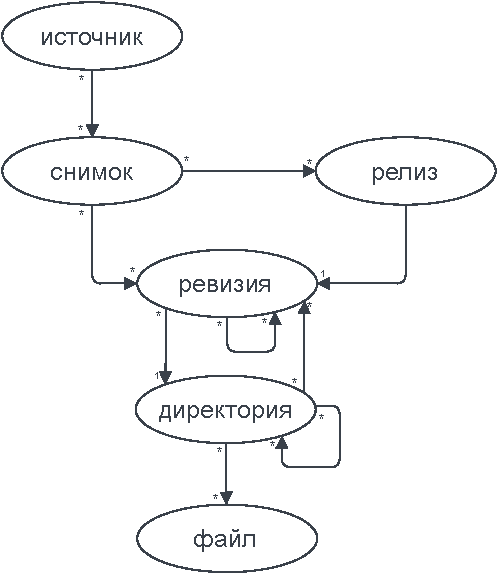
\includegraphics{img/swh-graph-structure.pdf}
\end{figure}

Единый граф архива содержит более 20 миллиардов вершин и более 230 миллиардов ребер~\cite{swh-dataset}. При таком крупном размере графа эффективное исполнение запросов на нем возможно при сжатии структуры графа, что позволяет разместить весь граф в менее чем ста гигабайтах оперативной памяти~\cite{saner}. При этом для сжатия структуры используется упомянутый ранее фреймворк WebGraph.

Архив Software Heritage содержит большое количество информации, анализ которой может представлять интерес. Веб-сервер Software Heritage предоставляет доступ к фиксированному набору запросов на графе, позволяющих анализировать информацию, хранящуюся в графе~\cite{swh-api}. Как было описано в разделе~\ref{sec:web-lim}, WebGraph предоставляет возможность осуществлять запросы к сжатому графу только в нативном виде~--- непосредственно используя методы, предоставляющие доступ к структуре графа. Это означает, что каждый предоставленный веб-сервером запрос потребовал непосредственной реализации на стороне сервера, а реализация нового запроса потребует вновь использовать лимитированные методы WebGraph. Для того чтобы упростить реализацию новых запросов к графу Software Heritage, а также стандартизировать подход к их реализации (вместо изучения методов WebGraph и реализации поверх них, может быть использован стандартный доменно-ориентированный язык), команда хочет изучить возможность использования языка Gremlin для этих нужд~\cite{swh-intern}. В случае успеха это позволит обрабатывать большой граф Software Heritage c удобством экспрессивного высокоуровнего языка, при этом сохранив эффективность исполнения запросов, достигаемую сжатием графа.

\section{Проверка производительности}

Поскольку TinkerPop предоставляет широкие возможности для обхода графов и в основном направлен на работу с графовыми базами данных, а WebGraph в свою очередь предоставляет весьма лимитированный набор методов, предоставляющих доступ к структуре графа, фокусируясь на оптимизации памяти, следует проверить, не внесет ли их связка проблем с производительностью, и убедиться, что решение имеет практическую пользу. Для этого потребуется провести анализ производительности, собрав данные об эффективности исполнения запросов, сравнив их с нативным реализациями.

\section{Постановка задачи}

Целью работы является реализация TinkerPop инфраструктуры для фреймворка для сжатия графов WebGraph. Это позволит выполнять сложные запросы на больших графах, используя язык Gremlin. Кроме того, необходимо добавить возможность указывать сторонние источники свойств вершин/ребер. После этого требуется сформулировать ряд запросов, анализ производительности исполнения которых покажет, насколько данный подход применим на практике.

\finishrelatedwork

\chapterconclusion
В первой главе была описана предметная область работы. Было показано, какая проблема существует, приведен пример случая, в котором решение этой проблемы будет актуально, а также разобраны альтернативные способы решения, и почему в этом случае они не подходят.

\chapter{Предлагаемый подход к задаче добавления поддержки Gremlin для WebGraph}

В данной главе будет описана общая структура решения, проведено разбиение на подзадачи, подробнее описаны детали каждой подзадачи. 

\section{Разбиение на подзадачи}

Исходя из постановки задачи можно выделить три отдельные подзадачи:

\begin{enumerate}
    \item Реализовать интерфейсы Apache TinkerPop, превращающие WebGraph в TinkerPop-enabled систему;
    \item Реализовать возможность указывать источники и способы доступа к свойствам вершин и ребер для использования этих свойств в запросах;
    \item Провести анализ производительности полученной реализации;
\end{enumerate}

Далее каждая из подзадач по отдельности будет рассмотрена подробнее.

\section{Реализация TinkerPop для WebGraph}

В данном разделе описывается общая архитектура решения, а также предложен метод взаимодействия между представлениями графа в TinkerPop и WebGraph.

\subsection{Общая архитектура}

Поскольку данная реализация нацелена на случай, в котором пользователь уже использует фреймворк WebGraph, а значит располагает представлением сжатого графа, и имеет возможность исполнять на нем нативные запросы, однако хочет получить возможность исполнять запросы и на Gremlin, следует рассматривать реализацию как библиотеку, получающую в том или ином виде сжатый WebGraph граф, и предоставляющую таким образом возможность исполнять на нем запросы на Gremlin, делегируя описанные выше методы лежащему в основе сжатому графу, с добавлением требуемой пред и постобработки аргументов и результатов.

\subsection{Структурные интерфейсы и методы TinkerPop}\label{tinkerpop-structure}

Как было описано в разделе~\ref{gremlin}, для получения возможности исполнять Gremlin запросы в собственной системе, требуется реализовать интерфейсы фреймворка Apache TinkerPop. Конкретнее, нужно реализовать интерфейсы пакета \texttt{/structure}, которые предоставляют абстракции для основных примитивов графовой модели данных~--- граф, вершина, ребро. Также, в этом пакете содержатся интерфейсы и методы для работы со свойствами, которые будут подробнее разобраны в разделе~\ref{props}.

Рассмотрим основные интерфейсы пакета \texttt{/structure}:

\begin{itemize}
    \item \texttt{Graph}~--- основной интерфейс графа. Экземпляр позволяет получать доступ к вершинам и ребрам по их идентификатору, либо ко всем вершинам и ребрам графа;
    \item \texttt{Vertex}~--- интерфейс вершины графа. Позволяет получить входящие и исходящие вершины и ребра, а также доступные свойства по их ключу;
    \item \texttt{Edge}~--- интерфейс ребра графа. Позволяет получить входящие и исходящие вершины, а также доступные свойства по их ключу;
    \item \texttt{Property}~--- интерфейс свойства вершины и ребра. Предоставляет доступ к значениям свойств;
\end{itemize}

Помимо описанных методов, TinkerPop предоставляет группы методов, поддержка которых реализовываться не будет:

\begin{itemize}
    \item Модифицирующие запросы~--- TinkerPop поддерживает запросы, модифицирующие граф. В данной реализации такие методы поддерживаться не будут, так как WebGraph не предоставляет возможности модифицировать граф во время работы с ним;
    \item Метасвойства вершин~--- TinkerPop поддерживает свойства вершин, являющиеся полноценными элементами графа, то есть имеющих свой уникальный идентификатор и свойства. В данной реализации такая возможность поддерживаться не будет, так как стандартной поддержки как мета, так и обычных свойств вершин WebGraph не предоставляет;
    \item Методы, специфичные для графовых баз данных~--- TinkerPop поддерживает методы, связаны со случаем использования в графовой базе данных, например \texttt{transaction()}. В данной реализации такая возможность поддерживаться не будет, так как в описываемом случае реализация основывается не на графовой базе данных;
\end{itemize}

Не стоит считать, что наличие подобных ограничений описываемого случая и, как следствие, отсутствие реализации указанных групп методов означает недостаточную совместимость TinkerPop и WebGraph. Как упоминалось в разделе~\ref{gremlin}, несмотря на то, что TinkerPop действительно в большей мере направлен на работу с графовыми базами данных, где указанные группы методов оправданы, TinkerPop является фреймворком общего назначения для любых графовых систем, и отсутствие реализации указанных групп методов является ожидаемым, что подтверждается наличием стандартных исключений для каждой описанной ранее группы методов, информирующих об отсутствии реализации этой группы в данной системе.

\subsection{Отличия графовых примитивов в WebGraph и TinkerPop}

Как было описано в разделе~\ref{tinkerpop-structure}, TinkerPop предоставляет абстракции для вершин и ребер, и работает с их экземплярами. WebGraph в свою очередь, предоставляет доступ только к вершинам, ссылаясь на их уникальный числовой идентификатор~--- индекс. Располагая индексом вершины можно получить итератор по индексам вершин-соседей. При этом отдельной абстракции для ребер в WebGraph нет. Это позволяет эффективно работать со структурой графа в памяти, однако усложняет работу с ней пользователю. Отличие в представлениях этих примитивов означает, что для реализации взаимодействия потребуется создавать объекты-обертки. Здесь можно рассмотреть два подхода:
\begin{enumerate}
    \item Сопоставить каждой вершине или ребру в WebGraph единственный объект, который будет возвращаться при любом доступе к данной вершине или ребру;
    \item Возвращать временные объекты при доступе к данной вершине или ребру~--- нет гарантии, что два различных запроса к одной вершине или ребру вернут один и тот же объект, однако гарантируется, что объекты будут равны и будут обладать одинаковыми свойствами;
\end{enumerate}

Первый вариант подразумевает создание единого реестра объектов для получения гарантии идентичности возвращаемых объектов при различных запросах. Учитывая цель сохранить преимущество в использовании памяти, получаемое за счет сжатия графа, этот подход не является лучшим выбором, так как создает дополнительную нагрузку на память, которая при участии в обходе достаточного числа вершин, станет существенной проблемой.
Второй подход в свою очередь удобен своей гибкостью. Оставляя возможность создавать новые объекты при каждом новом обращении к вершине, он не исключает возможности внесения оптимизаций для уменьшения общего числа аллокаций новых объектов.

\section{Работа со свойствами вершин и ребер графа}\label{props}

Вершины и ребра в графе могут обладать свойствами. Примером свойства вершины может быть название аэропорта для графа рейсов, а свойством ребра может являться расстояние между аэропортами.
Многие запросы к графовой структуре данных представляют интерес именно в привязке к свойствам и их значениям, так как без их учета запрос может опираться только на структуру графа. Примером запроса на графе рейсов, зависящего от свойств вершин, может являться самый ранний рейс по выбранному направлению. В данном случае время вылета будет свойством вершины, обозначающей рейс.

\subsection{Свойства в TinkerPop}

Gremlin предоставляет возможность формулировать запросы, зависящие от свойств. Свойства устроены как пара ключ-значение, где ключ является строкой, а значение объектом. Gremlin позволяет как проверять наличие свойства с данным ключом у данной вершины или ребра, так и получать  значение свойства, а также использовать это значение в самом запросе, например для фильтрации. С примером запроса, зависящего от свойств, можно ознакомиться на листинге~\ref{lst2}.

\begin{lstlisting}[float=!h,caption={Пример запроса на Gremlin, зависящего от свойств},label={lst2}]
g.V().where(values('terminals').is(gt(3)))
\end{lstlisting}

TinkerPop, в свою очередь, предоставляет интерфейс \texttt{Property}, который используется для получения доступа к свойствам данной вершины или ребра. Имеется возможность как получить доступ ко всем доступным свойствам вершины или ребра, так и к конкретным свойствам, предоставив список ключей этих свойств. Этот список будет являться фильтром для доступных у данной вершины или ребра свойств.

Помимо свойств, TinkerPop также вводит понятие <<меток>>. Вершины и ребра могут обладать единственной строковой меткой. Так как метка единственна, для получения доступа к ней не требуется предоставлять ключ. С диаграммой модели свойств в TinkerPop можно ознакомиться на рисунке~\ref{fig2}.

\begin{figure}[!h]
\caption{Архитектура свойств в TinkerPop}\label{fig2}
\centering
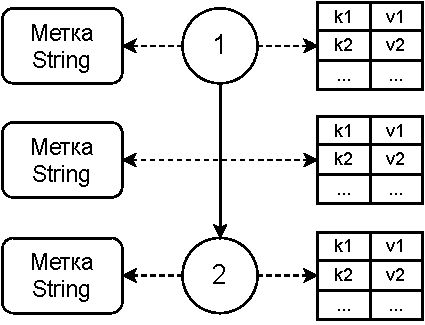
\includegraphics{img/tinker-props.pdf}
\end{figure}

\subsection{Свойства в WebGraph}\label{sec:webgraph-props}

WebGraph~--- фреймворк, сжимающий графы с точки зрения их структуры, поэтому поддержка работы со свойствами как таковая не является целью фреймворка. WebGraph предоставляет единственный способ работы со свойствами~--- по индексу вершины можно получить как индексы ее соседей, так и <<помеченных>> соседей, то есть пару из индекса соседа и <<метки>>.
Эти метки можно считать свойством ребра из изначальной вершины в соседа. Для каждого ребра можно хранить единственный объект метку. В остальном работа со свойствами перекладывается на пользователя, в частности свойства вершин или хранение нескольких свойств для ребер. Диаграмма модели свойств в WebGraph представлена на рисунке~\ref{fig3}.

\begin{figure}[!h]
\caption{Архитектура свойств в WebGraph}\label{fig3}
\centering
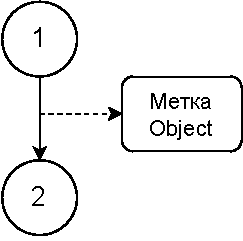
\includegraphics{img/webgraph-props.pdf}
\end{figure}

Тем не менее хранение свойств вершин и ребер, помимо самой структуры графа, является важной элементом работы с графом, ведь как обсуждалось в разделе~\ref{props}, запросы зачастую представляют интерес именно в привязке к свойствам. Поэтому существует ряд стандартных практик, использующихся для хранения и получения доступа к свойствам при работе с WebGraph.
К примеру для свойств вершин может использоваться сериализация массива примитивных значений, в котором индекс в массиве соответствует индексу вершины, а значение по индексу~--- значению свойства для соответствующей вершины. Следует реализовать ряд классов, позволяющих пользователю удобным образом задавать собственные способы хранения свойств, а также использовать стандартные.

\section{Анализ производительности реализации}

TinkerPop предоставляет широкие возможности для обхода графов, а также в основном используется в графовых базах данных. WebGraph в свою очередь фокусируется на достижении малого отпечатка в памяти, и используется в том случае, когда эффективность и минимальные накладные расходы критически необходимы.
При связке этих двух фреймворков могут возникнуть проблемы с производительностью~--- требуется как сохранить малый отпечаток в памяти, достигаемый сжатием графа, так и оценить, не становятся ли критическими накладные расходы, которые появляются при адаптации WebGraph к TinkerPop.

Чтобы провести анализ производительности, предлагается выбрать конкретный набор данных, представленный в виде графа. Следует определить ряд запросов, представляющих на нем интерес, после чего реализовать данные запросы на языке Gremlin, и, используя сжатое WebGraph представление данного графа и разработанную связку, исполнить данные запросы, проанализировав результаты по ряду метрик, таких как:

\begin{itemize}
    \item время выполнения;
    \item используемая память;
    \item число вершин и ребер, затронутых в процессе исполнения;
    \item число результатов;
\end{itemize}

Подобный анализ позволит оценить потерю в эффективности, вызванную разработанной связкой, и сделать выводы о практической применимости решения.

\chapterconclusion
В этой главе были подробнее рассмотрены конкретные шаги, необходимые для достижения поставленной задачи. Описаны основные интерфейсы WebGraph и TinkerPop, отличия в моделях свойств. Кроме того был описан подход к верификации решения.

\chapter{Реализация библиотеки, связывающей WebGraph и TinkerPop}

Фреймворк WebGraph реализован на языке Java, и так как решение нацелено на случай, в котором пользователь уже использует WebGraph, и желает получить возможность исполнять на доступном графе Gremlin запросы, решение также было реализовано на языке Java. TinkerPop также реализован на языке Java, что упрощает разработку взаимодействия двух фреймворков.

\section{Реализация TinkerPop}

В разделе~\ref{tinkerpop-structure} были описаны интерфейсы и методы, предоставляемые TinkerPop, реализация которых позволяет исполнять в ней Gremlin запросы (англ. TinkerPop-enabled system). Согласно конвенции реализации этих интерфейсов должны именоваться из двух частей: название системы и название интерфейса в качестве суффикса. В качестве названия системы естественным образом было решено использовать \texttt{WebGraph}. Далее эти интерфейсы и их реализации будут рассмотрены подробнее. 

\subsection{WebGraphGraph}

Интерфейс \texttt{Graph} является основной точкой входа TinkerPop. Согласно конвенции его реализация для определенной системы должна содержать публичный статический метод (или несколько методов), возвращающий экземпляр этого класса, и этот метод должен использоваться для создания объектов интерфейса \texttt{Graph}.
Для взаимодействия с WebGraph этот метод должен получать в качестве параметра класс, предоставляющий доступ к сжатому графу. На момент начала работы единственным подходящим классом был \texttt{ImmutableGraph}, позволяющий обходить граф в одном направлении.
Поскольку TinkerPop позволяет обходить граф как в прямом, так и в обратном направлении ребер, после консультации с командой WebGraph, во фреймворк был добавлен новый класс \texttt{BidirectionalImmutableGraph}~\cite{vigna-bidir}, позволяющий получать не только соседей по направлению ребер, но и соседей в обратном направлении. Именно этот класс будет использоваться как основная точка доступа к структуре сжатого графа, а методы TinkerPop будут делегироваться этому классу.

Помимо создания графа интерфейс \texttt{Graph} позволяет получать доступ к вершинам и ребрам графа по их идентификаторам, а также ко всем вершинам или ребрам.

\subsubsection{Получение вершин}

Доступ к вершинам в TinkerPop осуществляется через метод \texttt{vertices(Object... vertexIds)}, возвращающий итератор по вершинам с данными индексами, либо итератор по всем вершинам, если массив предоставленных индексов пустой.
Так как индексы вершин в WebGraph это числа типа \texttt{long}, ожидается, что будут предоставлены идентификаторы именно этого типа.
Для предоставленных индексов возвращаются объекты-обертки над ними класса \texttt{WebGraphVertex}, описанного в разделе~\ref{subsec:webgraphvertex}.
Если массив индексов пустой, обертки возвращаются над индексами, полученными методом \texttt{nodeIterator()} класса \texttt{ImmutableGraph}, возвращающем итератор по всем вершинам графа.

\subsubsection{Получение ребер}

Доступ к ребрам в TinkerPop осуществляется аналогично вершинам~--- метод \texttt{edges(Object... edgeIds)} возвращает итератор по ребрам с данными индексами, либо итератор по всем ребрам, если массив индексов пустой.
Так как абстракции над ребрами в WebGraph нет, идентификаторы ребер должны быть синтетическими. Поскольку WebGraph не поддерживает кратные ребра, в качестве такого идентификатора можно использовать пару индексов, обозначающих исходящую и входящую вершины. Для этого использовался класс \texttt{LongLongPair} библиотеки \texttt{fastutil}~\cite{fastutil}.
Для предоставленных индексов возвращаются объекты-обертки над ними класса \texttt{WebGraphEdge}, описанного в разделе~\ref{subsec:webgraphedge}.
Если массив индексов пустой, обертки возвращаются над индексами, в которых исходящая вершина получается методом \texttt{nodeIterator()} класса \texttt{ImmutableGraph}, а входящая вершина методом \texttt{successors(long vertexId)} со значением аргумента, равным индексу исходящей вершины, возвращающем итератор по индексам соседей исходящей вершины. Таким образом перебираются все начальные вершины, а для каждой начальной вершины все конечные. Все пары таких вершин описывают все ребра графа.

\subsection{WebGraphVertex}\label{subsec:webgraphvertex}

Интерфейс \texttt{Vertex} обозначает вершину графа. Он предоставляет доступ к идентификатору вершины, ее метке, лежащему в основе графу (эти три метода выделены в интерфейс \texttt{Element}), входящим и исходящим вершинам и ребрам, а также свойствам вершины.
Идентификатор и граф сопровождаются в конструкторе \texttt{WebGraphVertex}, о метках и свойствах речь пойдет в разделах~\ref{subsec:webgraphproperty} и~\ref{sec:props}.
Для получения вершин и ребер используются методы \texttt{successors(long vertexId)} и \texttt{predecessors(long vertexId)} класса \texttt{BidirectionalImmutableGraph}. Возвращаемый ими \texttt{LazyLongIterator} оборачивается в стандартный \texttt{Iterator} пакета \texttt{java.util}. При доступе к вершинам возвращаются обертки над индексом вершины-соседа, а при доступе к ребрам~--- обертки над парой индексов: текущей вершины и полученного соседа.

\subsection{WebGraphEdge}\label{subsec:webgraphedge}

Интерфейс \texttt{Edge} обозначает ребро графа. Он предоставляет доступ к описанным выше методам интерфейса \texttt{Element} (идентификатор, метка, граф), входящей и исходящей вершинам, а также свойствам ребра. Идентификатор и граф сопровождаются в конструкторе \texttt{WebGraphEdge}, о метках и свойствах речь пойдет в разделах~\ref{subsec:webgraphproperty} и~\ref{sec:props}.
Для входящей и исходящей вершин возвращаются обертки над их индексами.

\subsection{WebGraphProperty}\label{subsec:webgraphproperty}

Доступ к свойствам в TinkerPop осуществляется через метод \texttt{properties(String propertyKeys)} интерфейса \texttt{Element}, общего у \texttt{Vertex} и \texttt{Edge}, где \texttt{propertyKeys} являются фильтром над доступными свойствами. Если ключей предоставлено не было, возвращаются все доступные свойства.

Сам интерфейс \texttt{Property} является аналогом \texttt{Optional} пакета \texttt{java.util}, помимо значения обладающим дополнительным строковым ключом. Определяет методы для получения ключа, значения, проверки наличия значения. При этом как упоминалось в разделе~\ref{tinkerpop-structure}, TinkerPop поддерживает метасвойства вершин, поэтому для свойств вершин используется отдельный интерфейс \texttt{VertexProperty}, объединяющий интерфейсы \texttt{Property} и \texttt{Element}. В рамках работы добавление поддержки метасвойств не планируется, поэтому методы получения свойств для класса \texttt{WebGraphVertexProperty} вызывают стандартное исключение \texttt{VertexProperty.Exceptions.metaPropertiesNotSupported()}.

В классах \texttt{WebGraphVertex} и \texttt{WebGraphEdge} реализация метода \texttt{properties(String propertyKeys)} получает доступные свойства и их значения через класс \texttt{WebGraphPropertyProvider}, речь о котором пойдет в разделе~\ref{sec:provider}. Пользуясь либо предоставленными ключами, либо списком всех доступных ключей, возвращается итератор по оберткам свойств с отфильтрованными \texttt{null} значениями.

\section{Реализация работы со свойствами}\label{sec:props}

Модели свойств в TinkerPop и WebGraph заметно отличаются. Более того, поддержка свойств при работе с WebGraph во многом ложится на самого пользователя. Чтобы наладить взаимодействие между этими моделями свойств, а также упростить работу со стандартными подходами к хранению свойств в WebGraph, был разработан ряд классов, речь о которых пойдет далее. Схема архитектуры свойств представлена на рисунке~\ref{props-diagram}.

\begin{figure}[!h]
\caption{Общая схема архитектуры свойств}\label{props-diagram}
\centering
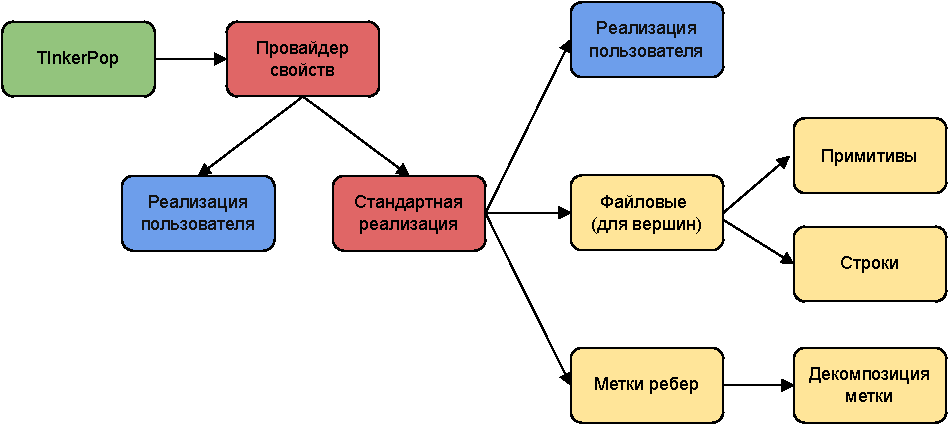
\includegraphics{img/props.pdf}
\end{figure}

\subsection{Провайдер свойств}\label{sec:provider}

Интерфейс \texttt{WebGraphPropertyProvider} отвечает за доступ к меткам вершин и ребер, доступным ключам свойств, а также к значениям этих свойств. Он является связующим звеном между моделью свойств в TinkerPop и работой со свойствами в WebGraph. Экземпляр этого интерфейса наравне с экземпляром \texttt{BidirectionalImmutableGraph} необходим для создания \texttt{WebGraphGraph}.

\subsection{Стандартный провайдер свойств}

Пользователь может как предоставить свою реализацию \texttt{WebGraphPropertyProvider}, так и использовать стандартную \texttt{StandardWebGraphPropertyProvider}. Стандартная реализация позволяет определять метки вершин и ребер, предоставив функцию из индекса в строковую метку, а также регистрировать свойства при помощи отдельных классов \texttt{VertexProperty} и \texttt{EdgeProperty}. Конструкторы этих классов принимают строковый ключ свойства, а также функцию, возвращающую значение по идентификатору вершины или ребра.
Эти свойства регистрируются в провайдере. Метод, возвращающий доступные ключи, возвращает ключи всех зарегистрированных свойств. По ключу свойства и идентификатору вершины или ребра провайдер обращается к соответствующему зарегистрированному свойству и возвращает полученное значение. Провайдер имеет доступ ко всем зарегистрированным свойствам, поэтому при попытке регистрации свойства с занятым ключом, пользователь получает сообщение о том, что свойство с данным ключом уже существует.

\subsection{Стандартные свойства вершин}

Как упоминалось в разделе~\ref{sec:webgraph-props}, WebGraph не предоставляет стандартных методов работы со свойствами вершин~--- эта задача перекладывается на пользователя. При этом пользователи зачастую используют ряд стандартных практик для работы с ними. Чтобы упростить работу со свойствами в разрабатываемой связке, часть таких стандартных практик была реализована. Пользователь имеет возможность определять свои \texttt{VertexProperty}, однако если он решает воспользоваться одним из стандартных методов, от него потребуется минимальная настройка. Далее будут подробнее разобраны стандартные подходы и их реализации. 

\subsubsection{Файловые свойства вершин}

Поскольку WebGraph не поддерживает свойства вершин, чаще всего пользователи сохраняют их в отдельных файлах вместе со структурой графа. Удобным способом хранения свойств вершин является хранение массива значений в сериализованном виде. Индекс в массиве соответствует индексу вершины, а значение по индексу~--- значению свойства для соответствующей вершины. Для сохранения и чтения массива хорошо подходит библиотека \texttt{fastutil} от создателей WebGraph. Она уже используется в самом фреймворке WebGraph и ее использование напрашивается и для работы со свойствами.
Эта библиотека позволяет сериализовывать и читать из файла массивы примитивов, что дает возможность определить файловые свойства вершин для всех примитивов. Для этого был создан класс \texttt{FileVertexProperty}, принимающий ключ свойства, тип значения и путь к файлу с массивом сериализованных значений. По типу свойства класс выбирает нужный способ чтения файла и позволяет получать доступ к значениям.

Помимо примитивов, важным типом свойств является строковый тип, так как многие данные для вершин и ребер имеют именно текстовое представление. Для того чтобы добавить поддержку строковых свойств вершин и ребер, был реализован следующий метод хранения. В первом файле хранится буфер~--- байтовый массив блоков, каждый из которых соответствует отдельной строке. Каждый блок состоит из двух частей: первые 4 байта хранят число $n$~--- длину строки, а последующие $n$ байт~--- саму строку в байтовом представлении. Во втором массиве типа \texttt{long} хранятся сдвиги для каждой из вершин~--- ссылка на индекс начала нужного блока в буфере. Чтобы получить значение строки для данной вершины, следует сначала получить соответствующий вершине сдвиг, затем по индексу данного сдвига прочитать первые 4 байта блока, получив длину строки $n$, а затем считать последующие $n$ байт блока~--- байтовый массив самой строки. Воспользовавшись конструктором \texttt{String(byte[] bytes)} можно получить связанную с данной вершиной строку. С диаграммой данного метода можно ознакомиться на рисунке~\ref{fig:blocks}. 
Описанный механизм реализован в классе \texttt{StringFileVertexPropertyGetter}, конструктор которого принимает пути к файлам с буфером и сдвигами и позволяет получить доступ к значениям.

\begin{figure}[!h]
\caption{Хранение строкового свойства вершины}\label{fig:blocks}
\centering
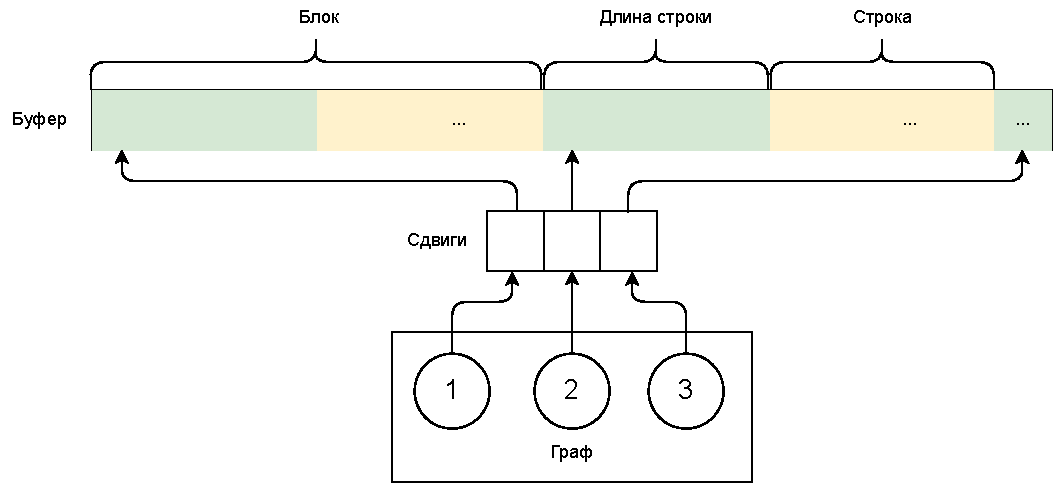
\includegraphics[width=\textwidth]{img/blocks.pdf}
\end{figure}

\subsection{Стандартные свойства ребер}

Как обсуждалось в разделе~\ref{sec:webgraph-props}, WebGraph поддерживает один способ указания свойств ребер~--- метки ребер. Помимо метода \texttt{sucessors(long vertexId)}, возвращающего итератор по соседям вершины, есть также метод \texttt{labelledSucessors(long vertexId)}, доступный у класса \texttt{ArcLabelledImmutableGraph} и возвращающий итератор по помеченным соседям. Таким образом метка соседа является меткой ребра из изначальной вершины в соседа. Каждое ребро может обладать одной меткой типа \texttt{Object}. В разработанной библиотеке пользователь имеет возможность определять свои \texttt{EdgeProperty}, однако для меток ребер был разработан отдельный класс, упрощающий работу с ними.

\subsubsection{ArcLabelEdgeProperty}

Для того чтобы предоставить TinkerPop доступ к меткам ребер, был разработан класс \texttt{ArcLabelEdgeProperty}. В конструкторе он принимает экземпляр помеченного графа \texttt{ArcLabelledImmutableGraph}, к которому должен иметь доступ пользователь, если он работает с метками в WebGraph. Чтобы получить метку ребра из вершины $a$ в вершину $b$ берется итератор по помеченным соседям вершины $a$, находится ребро в вершину $b$ и берется его метка. Поскольку подобное свойство у графа может быть только одно, оно обладает зарезервированным ключом. Это предотвращает возможность зарегистрировать одно и то же свойство под разными ключами.

Поскольку метка единственна для ребра, зачастую хранение нескольких свойств реализовывается за счет хранения нескольких полей в объекте метки, где каждое поле отвечает за отдельное свойство. Для того чтобы предоставить возможность декомпозировать метку на несколько свойств с различными ключами, минуя необходимость декомпозировать метку самостоятельно в каждом Gremlin запросе, был добавлен класс \texttt{ArcLabelEdgeSubProperty}, принимающий в конструкторе ключ свойства и функцию, отбирающую требуемое значение из полной метки. В реализации это свойство обращается к полной метке и возвращает результат применения функции к объекту метки. С примером использования декомпозиции метки можно ознакомиться на листинге~\ref{lst:arclabel}. Помимо декомпозиции метки этот класс также дает возможность создавать синтетические свойства, то есть произвольные трансформации над изначальной меткой. К примеру таким образом можно объединить два поля в одно отдельное свойство.


\begin{lstlisting}[float=!h,caption={Пример декомпозиции метки},label={lst:arclabel}]
var arcLabel = new ArcLabelEdgeProperty<MyArcLabel>(myGraph.getLabelledGraph());
p.addEdgeProperty(new ArcLabelEdgeSubProperty<>("duration", arcLabel, MyArcLabel::getDuration));
\end{lstlisting}

\section{Исполнитель запросов}\label{sec:executor}

Для того чтобы предоставить пользователю возможность запускать Gremlin запросы на графе, был разработан класс \texttt{GremlinQueryExecutor}, принимающий в конструкторе экземпляр интерфейса \texttt{Graph} (подразумевается, что это будет объект класса \texttt{WebGraphGraph}), и предоставляющий набор методов для запуска запросов на этом графе. Базовым методом является метод \texttt{eval(String query)} (реализация представлена на листинге~\ref{lst:gremlin-eval}), делегирующий исполнение запроса классу \texttt{GremlinExecutor} из пакета \texttt{org.apache.tinkerpop.gremlin.groovy.engine}.

\begin{lstlisting}[float=!h,caption={Реализация исполнителя Gremlin запросов},label={lst:gremlin-eval}]
public GraphTraversal<?, ?> eval(String query) {
    Bindings bindings = new SimpleBindings();
    bindings.put("g", g.traversal());
    try (GremlinExecutor ge =
                 GremlinExecutor.build()
                                .globalBindings(bindings)
                                .create()) {
        return (GraphTraversal<?, ?>) ge.eval(query, bindings).get();
    } catch (Exception e) {
        throw new RuntimeException(e);
    }
}
\end{lstlisting}

Для удобства работы с результатами запросов были добавлены два вспомогательных метода. \texttt{print(String query)} выводит в консоль все результаты запроса по мере исполнения, а \texttt{get(String query)} возвращает список результатов для дальнейшего использования в программе.

Для профилирования запросов Gremlin предоставляет стандартный шаг \texttt{profile()}. Для удобства профилирования в исполнитель запросов был добавлен метод \texttt{profile(String query)}, добавляющий этот шаг к изначальному запросу. Помимо этого, для работы с запросами, исполнение которых занимает заметное время, был добавлен метод \texttt{time(String query, long total)}, принимающий запрос и ожидаемое число результатов, и по ходу исполнения запроса выводящий в консоль статистику: число обработанных результатов, скорость обработки и прогноз оставшегося времени исполнения.

Gremlin предоставляет возможность формулировать запросы не только в качестве строк, но и при помощи классов и методов (англ. Gremlin-Java DSL). Это позволяет проводить статистический анализ запросов, в том числе типов, делает возможным автодополнение и использование \texttt{javadoc} для шагов, что упрощает формулировку запросов. Запрос, сформулированный таким образом, представлен классом \texttt{GraphTraversal}, а стартовой точкой является класс \texttt{GraphTraversalSource}. Все описанные выше методы класса \texttt{GremlinQueryExecutor} имеют аналог, принимающий в качестве аргумента не строковый запрос, а функцию из \texttt{GraphTraversalSource} в \texttt{GraphTraversal}, тем самым позволяя запускать запросы, сформулированные на Gremlin-Java DSL. С примерами запуска идентичных запросов, сформулированных с применением двух описанными подходов, можно ознакомиться на листингах~\ref{lst:gremlin-str} и~\ref{lst:gremlin-dsl}.

\begin{lstlisting}[float=!h,caption={Строковый Gremlin  запрос},label={lst:gremlin-str}]
executor.print("g.V().not(in())");
\end{lstlisting}

\begin{lstlisting}[float=!h,caption={Запрос на Gremlin-Java DSL},label={lst:gremlin-dsl}]
executor.print(g -> g.V().not(in()));
\end{lstlisting}

\section{Использование разработанной библиотеки}

Решение было реализовано в качестве Java библиотеки \texttt{webgraph-tinkerpop}. Пользователь, уже использующий WebGraph в своей системе, имеет возможность добавить разработанную библиотеку в зависимости, после чего он получает доступ к конструктору \texttt{WebGraphGraph}, классам для работы со свойствами, и исполнителю Gremlin запросов \texttt{GremlinQueryExecutor}.

Библиотека опубликована на хостинге GitHub и доступна по ссылке \url{https://github.com/andrey-star/webgraph-tinkerpop}. Библиотека не опубликована в центральном репозитории Maven~\cite{maven}, поэтому для добавления в зависимости своего проекта требуется скачать репозиторий и установить библиотеку в локальный Maven репозиторий при помощи команды \texttt{mvn install}, вызванной в корневой директории скачанного проекта. Для добавления самой зависимости требуется отредактировать файл \texttt{pom.xml} своего проекта и добавить в раздел \texttt{dependencies} строки, приведенные на листинге~\ref{lst:maven-dep}

\begin{lstlisting}[float=!h,caption={Добавление \texttt{webgraph-tinkerpop} в зависимости проекта},label={lst:maven-dep}]
<dependency>
    <groupId>org.webgraph.tinkerpop</groupId>
    <artifactId>webgraph-tinkerpop</artifactId>
    <version>1.0-SNAPSHOT</version>
</dependency>
\end{lstlisting}

С примером использования библиотеки для регистрации свойств и исполнения Gremlin запросов на графе можно ознакомиться на листинге~\ref{lst:webgraph-tinkerpop-example}.

\begin{lstlisting}[float=!h,caption={Пример использования библиотеки для регистрации свойств и исполнения Gremlin запросов},label={lst:webgraph-tinkerpop-example}]
var p = new StandardWebGraphPropertyProvider();
p.setVertexLabeller(myGraph::getNodeType);
p.addVertexProperty(new FileVertexProperty<>("timestamp", Long.class, Path.of("timestamp.bin")));
p.addVertexProperty(new VertexProperty<>("name", myGraph::getName));

var arcLabel = new ArcLabelEdgeProperty<MyArcLabel>(myGraph.getLabelledGraph());
p.addEdgeProperty(arcLabel);
p.addEdgeProperty(new ArcLabelEdgeSubProperty<>("duration", arcLabel, MyArcLabel::getDuration));

try (var gremlinGraph = WebGraphGraph.open(myGraph, p, myGraph.getPath())) {
    GremlinQueryExecutor executor = new GremlinQueryExecutor(gremlinGraph);
    executor.print(g -> g.V().has("timestamp", gt(1000)));
    executor.print("g.V().hasLabel('REV')");
}
\end{lstlisting}

\section{Внедрение результатов в проект Software Heritage}

Библиотека была использована для того, чтобы добавить возможность запускать Gremlin запросы на графе Software Heritage. Для этого в репозиторий \texttt{swh-graph}~\cite{swh-graph} была добавлена зависимость на разработанную библиотеку \texttt{webgraph-tinkerpop}.

Сервер Software Heritage уже имеет доступ к \texttt{BidirectionalImmutableGraph}, дополнительно обернутый в класс \texttt{SwhBidirectionalGraph}, поэтому для успешного использования библиотеки на том же сервере остается настроить использование свойств и получить экземпляр \texttt{WebGraphGraph} при помощи статического метода, описанного выше.

Для настройки свойств использовался класс \texttt{StandardWebGraphPropertyProvider}. В качестве метки вершины использовался тип вершины, получаемый методом \texttt{getNodeType(long vertexId)} класса \texttt{SwhBidirectionalGraph}. Меток ребер (имеются в виду строковых метки TinkerPop, не метки ребер WebGraph) рассматриваемый домен не предусматривает. Для добавления свойства вершины \texttt{author\_timestamp} использовался класс \texttt{FileVertexProperty}. Также были добавлены два свойства вершины, не подходящие под стандартные техники, и напрямую предоставляемые классом \texttt{SwhBidirectionalGraph}. Для этого использовался класс \texttt{VertexProperty}.
Для добавления свойства ребра был использован класс \texttt{ArcLabelEdgeProperty}, не требующий никаких настроек, достаточно предоставить \texttt{ArcLabelledImmutableGraph}. Также было добавлено дополнительное свойство поверх свойства ребра, конвертирующее набор файлов, связанных с ребром, в пары из строкового представления файла и числовой репрезентации прав доступа. Добавление этих свойств приведено на листинге~\ref{lst:props}.

\begin{lstlisting}[float=!h,caption={Добавление свойств для графа Software Heritage},label={lst:props}]
StandardWebGraphPropertyProvider provider = new StandardWebGraphPropertyProvider();
provider.setVertexLabeller(id -> graph.getNodeType(id).toString());
provider.addVertexProperty(new FileVertexProperty<>("author_timestamp", Long.class, Path.of(path + ".property.author_timestamp.bin")));
provider.addVertexProperty(new VertexProperty<>("swhid", graph::getSWHID));
provider.addVertexProperty(new VertexProperty<>("message", nodeId -> {
    try {
        return graph.getProperties().getMessage(nodeId);
    } catch (IOException e) {
        throw new UncheckedIOException(e);
    }
}));
ArcLabelEdgeProperty<DirEntry[]> edgeProperty = new ArcLabelEdgeProperty<>(graph.getForwardGraph().underlyingLabelledGraph());
provider.addEdgeProperty(edgeProperty);
provider.addEdgeProperty(new ArcLabelEdgeSubProperty<>("dir_entry_str", edgeProperty, SwhProperties::dirEntryStr));
\end{lstlisting}

\chapterconclusion

В третьей главе были подробно рассмотрены детали реализации TinkerPop для WebGraph, а именно исполнитель Gremlin запросов, взаимодействие структурных методов, а также моделей свойств двух фреймворков. Были описаны подходы к работе со свойствами в WebGraph и рассказано, каким образом эти методы были реализованы в библиотеке. В конце был приведен пример практического использования библиотеки командой Software Heritage.

\chapter{Проверка производительности библиотеки, связывающей WebGraph и TinkerPop}

Для проверки эффективности разработанной библиотеки был выбран реальный набор данных, в нем сформулированы представляющие интерес запросы. Эти запросы были реализованы на Gremlin, а также в нативном виде, после чего было проведено сравнение исполнения запросов по различным метрикам. В этой главе будет подробнее описан процесс тестирования и представлены его результаты.

\section{Набор данных}

В качестве домена был выбран архив Software Heritage, содержащий данные систем контроля версий репозиториев с открытым исходным кодом. Единый граф Software Heritage содержит более 20 миллиардов вершин и более 230 миллиардов ребер. Со структурой графа можно ознакомиться на рисунке~\ref{fig1}. Для тестов был выбран набор данных \texttt{python3k}~\cite{swh-dataset}, являющийся частью основного, и содержащий данные о трех тысячах популярных репозиториев на языке Python. Граф содержит 46 миллионов вершин и 1 миллиард 218 миллионов ребер. Software Heritage использует WebGraph для сжатия структуры графа, поэтому набор данных содержит все необходимые для работы с WebGraph файлы.

\section{Формулировка запросов}

Были сформулированы три запроса, представляющих интерес в данном домене:

\begin{itemize}
    \item Самая ранняя ревизия для файла или директории;
    \item Список файлов ревизии;
    \item Дерево ревизий снимка;
\end{itemize}

\subsection{Самая ранняя ревизия для файла или директории}

Принимая в качестве аргумента индекс файла или директории, этот запрос находит все ревизии, достижимые из этого файла или директории, и возвращает минимальную ревизию по значению свойства \texttt{author\_timestamp}. Таким образом результатом запроса является первая ревизия, в которой данный файл или директория появились в том виде, в котором они представлены в вершине, являющейся аргументом запроса. Область запроса представлена на рисунке~\ref{ecr-graph}.

\begin{figure}[!h]
\caption{Область графа, затрагиваемая запросом <<Первая ревизия файла или директории>>}\label{ecr-graph}
\centering
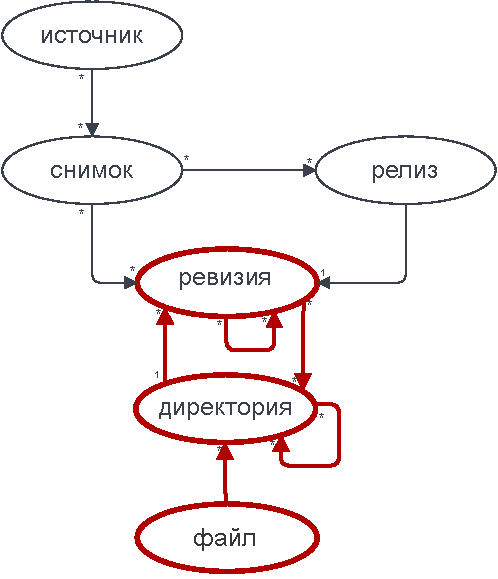
\includegraphics{img/ecr-graph.pdf}
\end{figure}

\subsection{Список файлов ревизии}

Принимая на вход в качестве аргумента индекс ревизии или директории, этот запрос возвращает пути и права доступа для всех доступных файлов и директорий данной ревизии или директории. Таким образом этот запрос является аналогом команды \texttt{ls -lR}. Названия директорий и файлов хранятся в метке ребра. Область запроса представлена на рисунке~\ref{rec-graph}.

\begin{figure}[!h]
\caption{Область графа, затрагиваемая запросом <<Список файлов ревизии>>}\label{rec-graph}
\centering
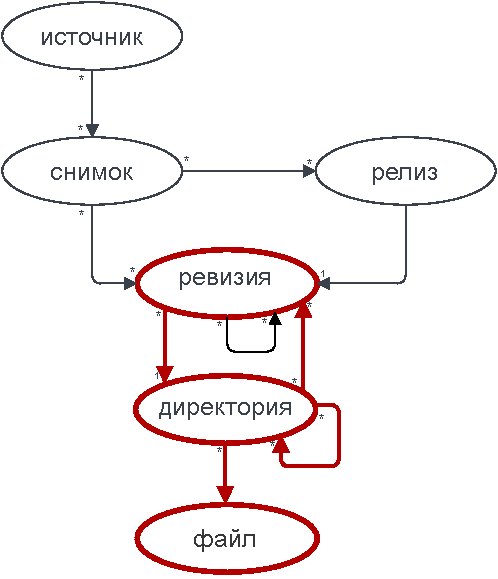
\includegraphics{img/rec-graph.pdf}
\end{figure}

\subsection{Дерево ревизий снимка}

Принимая на вход в качестве аргумента индекс снимка, этот запрос возвращает все связи между снимками, ревизиями и релизами. При этом, если ребро следует из снимка в ревизию, то эта связь представляет ветку, и результат сопровождается ее названием. Если ребро следует из снимка в релиз, то результат сопровождается названием релиза. Названия веток и релизов хранятся в метке ребра. Область запроса представлена на рисунке~\ref{snp-graph}.

\begin{figure}[!h]
\caption{Область графа, затрагиваемая запросом <<Дерево ревизий снимка>>}\label{snp-graph}
\centering
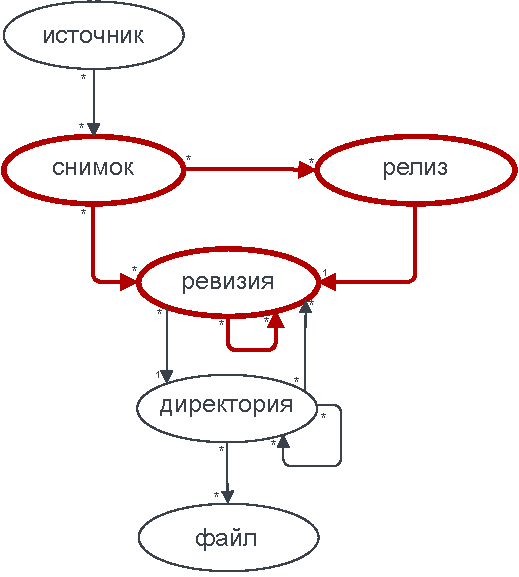
\includegraphics{img/snp-graph.pdf}
\end{figure}

\section{Реализация запросов на Gremlin}

Для того чтобы протестировать разработанную библиотеку на описанных запросах, требуется предварительно реализовать их на Gremlin. Запросы на Gremlin представляют собой цепочки <<шагов>>. Каждый шаг либо оперирует с результатами, полученными на предыдущем шаге, либо совершает стороннее действие (англ. side effect). Также существует два стартовых шага \texttt{V()} и \texttt{E()}, возвращающих вершины и ребра графа соответственно, опционально принимая идентификаторы интересующих вершин или ребер. Подробнее с доступными шагами и их действиями можно ознакомиться в документации к Gremlin~\cite{gremlin-steps}. Далее будут представлены и прокомментированы реализации трех описанных запросов.

\subsection{Самая ранняя ревизия для файла или директории}

Реализация запроса представлена на листинге~\ref{lst:ecr}.
\begin{enumerate}
    \item начинаем в файле или директории;
    \item рекурсивно переходим в предка, пропуская посещенные вершины;
    \item сохраняем все встреченные ревизии;
    \item избавляемся от повторений;
    \item сортируем по значению свойства \texttt{author\_timestamp} и берем первый результат;
\end{enumerate}

\begin{lstlisting}[float=!h,caption={Самая ранняя ревизия для файла или директории на Gremlin},label={lst:ecr}]
g.V(v)                                               // а
 .repeat(in().dedup())                               // б
 .emit(hasLabel("REV"))                              // в
 .dedup()                                            // г
 .order().by("author_timestamp", Order.asc).limit(1) // д
\end{lstlisting}

\subsection{Список файлов ревизии}

Реализация запроса представлена на листинге~\ref{lst:rec}.
\begin{enumerate}
    \item начинаем в ревизии или директории;
    \item если стартовая вершина это ревизия, переходим в соответствующую директорию;
    \item рекурсивно переходим в потомка, сохраняя пройденное ребро;
    \item для подмодулей переходим в соответствующую директорию;
    \item возвращаем каждую пройденную вершину;
    \item для каждой вершины рассматриваем весь пройденный до нее путь;
    \item для ребер на пути возвращаем свойство \texttt{dir\_entry\_str};
    \item совершаем постобработку свойств;
\end{enumerate}

\begin{lstlisting}[float=H,caption={Список файлов ревизии на Gremlin},label={lst:rec}]
g.V(root)                                        // а
 .choose(hasLabel("REV"), out().hasLabel("DIR")) // б
 .repeat(outE()                                  // в
           .inV().choose(hasLabel("REV"), out().hasLabel("DIR"))) // г
 .emit()                                         // д
 .path()                                         // е
 .map(unfold()
        .<SwhProperties.DirEntryString[]>values("dir_entry_str") // ж
        .fold()
 .flatMap(path -> {                              // и
     List<SwhProperties.DirEntryString[]> pathDirs = path.get();
     StringBuilder dir = new StringBuilder();
     for (int i = 0; i < pathDirs.size() - 1; i++) {
         dir.append(pathDirs.get(i)[0].filename) // parent path should not have duplicate edges
            .append("/");
     }
     SwhProperties.DirEntryString[] last = pathDirs.get(pathDirs.size() - 1);
     if (last.length == 1) {
         var entry = last[0];
         return List.of(String.format("%s%s [perms: %s]", dir, entry.filename, entry.permission))
                    .iterator();
     }
     List<String> res = new ArrayList<>();
     for (SwhProperties.DirEntryString entry : last) {
         res.add(String.format("%s%s [perms: %s]", dir, entry.filename, entry.permission));
     }
     return res.iterator();
 })
\end{lstlisting}

\subsection{Дерево ревизий снимка}

Реализация запроса представлена на листинге~\ref{lst:snp}.
\begin{enumerate}
    \item рекурсивно переходим в потомка, пропуская посещенные ребра;
    \item оставляем только ребра, оканчивающиеся ревизией или снимком;
    \item сохраняем оставшиеся ребра;
    \item переходим в оставшиеся ребра, избегая повторений;
    \item возвращаем множество встреченных ребер;
    \item конвертируем список ребер в индивидуальные ребра;
    \item получаем значение свойства, хранящего названия веток или релизов;
    \item конвертируем ребра во все доступные ветки или релизы;
\end{enumerate}

\begin{lstlisting}[float=!h,caption={Дерево ревизий снимка на Gremlin},label={lst:snp}]
g.withSideEffect("e", new HashSet<>())
 .V(snapshot)
 .repeat(outE().where(P.without("e"))                // а
           .where(inV().hasLabel("REV", "REL"))      // б
           .aggregate("e")                           // в
           .inV().dedup()                            // г
 .<Edge>cap("e")                                     // д
 .unfold()                                           // е
 .elementMap("filenames")                            // ж
 .flatMap(edgeElementMapTraverser -> {               // и
     Map<Object, Object> edgeElementMap = edgeElementMapTraverser.get();
     long outId = (long) ((Map<Object, Object>) edgeElementMap.get(Direction.OUT)).get(T.id);
     long inId = (long) ((Map<Object, Object>) edgeElementMap.get(Direction.IN)).get(T.id);
     String outLabel = (String) ((Map<Object, Object>) edgeElementMap.get(Direction.OUT)).get(T.label);

     String edgeStr = String.format("(%s -> %s)", outId, inId);
     if (outLabel.equals("SNP")) {
         String[] branches = (String[]) edgeElementMap.get("filenames");
         List<String> res = new ArrayList<>(branches.length);
         for (String branch : branches) {
             res.add(edgeStr + " " + branch);
         }
         return res.iterator();
     }
     return List.of(edgeStr).iterator();
 })
\end{lstlisting}

\section{Проведение тестирования}

Для измерения производительности запросов был разработан класс \texttt{Benchmark}, запускающий и профилирующий описанные запросы на случайном наборе подходящих вершин. 

Для этого был создан интерфейс \texttt{BenchmarkQuery}, определяющий ряд методов, необходимых профайлеру для измерений показателей запроса, а именно:

\begin{itemize}
    \item \texttt{getName()}~--- возвращает уникальный строковый идентификатор этого запроса;
    \item \texttt{getQuery()}~--- возвращает запрос, реализованный на Gremlin-Java DSL;
    \item \texttt{generateStartingPoints()}~--- возвращает случайный набор подходящих стартовых вершин для данного запроса;
    \item \texttt{nativeImpl(long id)}~--- нативная реализация этого запроса;
\end{itemize}

Этот интерфейс был реализован для каждого из трех запросов. Поскольку все три запроса имеют стартовой точкой вершину с определенной меткой, генерация случайных стартовых вершин осуществляется через предварительный Gremlin запрос, находящий вершины с этой меткой, а затем выбирающий случайный набор среди этих вершин. С реализацией этого запроса можно ознакомиться на листинге~\ref{lst:gremlin-rnd}.

\begin{lstlisting}[float=!h,caption={Генерация случайных стартовых вершин},label={lst:gremlin-rnd}]
private List<Long> randomVerticesWithLabel(String label, long count) {
    return e.get(g -> g.V().hasLabel(label)
                       .order().by(Order.shuffle)
                       .limit(count)
                       .id().map(id -> (long) id.get()));
}
\end{lstlisting}

Для анализа производительности профайлер генерирует стартовые точки для выбранного запроса, запускает запрос на этих стартовых точках и подводит статистику по мере исполнения. Так как время исполнения одного запроса может варьироваться, каждый запрос исполняется определенное число раз, а результат усредняется. Также исполняется и нативная версия запроса для проведения последующего сравнения.

Класс \texttt{Benchmark} принимает в качестве аргументов командной строки ряд параметров, позволяющих настраивать профайлер:

\begin{itemize}
    \item \texttt{graphPath}~--- путь к Software Heritage графу, на котором будут исполняться запросы;
    \item \texttt{query}~--- строковый идентификатор запроса, который следует профилировать;
    \item \texttt{samples}~--- число сгенерированных стартовых точек, на которых будет запускаться запрос;
    \item \texttt{iters}~--- число запусков запроса для одной стартовой точки;
    \item \texttt{argument}~--- при наличии пропускается генерация стартовых точек, вместо этого запрос исполняется для переданного аргумента;
    \item \texttt{print}~--- при наличии вместо промежуточных результатов профайлинга выводятся результаты запроса;
\end{itemize}

По мере исполнения профайлер выводит текущий аргумент и итерацию, время исполнения Gremlin запроса и нативного запроса, а также число результатов запроса. Для определения времени исполнения запроса и числа результатов используется описанный в разделе~\ref{sec:executor} шаг \texttt{profile()}. Также выводится скорость исполнения исходя из общего времени и числа результатов. Промежуточный вывод профайлера представлен на листинге~\ref{lst:bench-query}.

\begin{lstlisting}[float=!h,caption={Пример промежуточного вывода профайлера},label={lst:bench-query}]
Running query for id: 45673752 (92/100)
Native time: 506ms
1/3 Finished in: 2428ms. Results: 137874
2/3 Finished in: 2623ms. Results: 137874
3/3 Finished in: 2472ms. Results: 137874
Average for id: 45673752 - 2507ms. Per element: 0.02ms (137874 elements).
\end{lstlisting}

После окончания исполнения выводится общая статистика, такая как: среднее время исполнения запроса, средняя скорость исполнения относительно числа результатов, максимальное время исполнения и соответствующая стартовая точка, а также среднее время и скорость для нативной версии запросов, и коэффициент замедления Gremlin версии по сравнению с нативной. Текстовое представление результата шага \texttt{profile()} сохраняется в текстовые файлы для каждого запроса и итерации, что позволяет подробнее анализировать отдельные случаи. Числовые данные сохраняются в сводную таблицу в формате CSV для возможности дальнейшего анализа и построения графиков. С финальным выводом профайлера можно на листинге~\ref{lst:bench-summary}.

\begin{lstlisting}[float=!h,caption={Пример финального вывода профайлера},label={lst:bench-summary}]
Average time: 46ms. Per element: 0.02ms
Max time: 2507ms for id 45673752. Per element: 0.02ms (137874 elements)
Native time: 28ms. Per element: 0.01ms
Slower by: 1.63 times
Results saved at: benchmarks/2022-05-11T12:36:39Z-snapshotRevisionsWithBranches
\end{lstlisting}

\section{Результаты тестирования}

По результатам тестирования можно сделать выводы о том, какое замедление испытывает запрос по сравнению с его нативной реализацией. Хорошей метрикой для оценки этого показателя является скорость обработки элементов. Под число элементом стоит понимать некую оценку мощности запроса. Для многих запросов подходящим числом элементов может служить число результатов запроса, например для запросов <<Список файлов ревизии>> и <<Дерево ревизий снимка>>. Однако для некоторых запросов такая метрика не подходит, например у запроса <<Самая ранняя ревизия для файла или директории>> всего один результат. В этом случае можно использовать другое число, отражающее мощность запроса, например число пройденных вершин.

Для наглядного сравнения подходов были построены графики скорости обработки элементов. График для запроса <<Самая ранняя ревизия для файла или директории>> представлен на рисунке~\ref{fig-ecr}, для запроса <<Список файлов ревизии>> на рисунке~\ref{fig-rec}, для запроса <<Дерево ревизий снимка>> на рисунке~\ref{fig-snp}. На них отображена зависимость времени исполнения запроса от числа элементов для среднего по трем запускам Gremlin запроса, и нативного запуска запроса. Для удобства помимо графика нативного запуска добавлен график нативного запуска с коэффициентом, максимально приближенный к среднему запуску Gremlin. Это позволяет наглядно отобразить коэффициент замедления.

\begin{figure}[!h]
\caption{График зависимости времени исполнения запроса от числа элементов для запроса <<Самая ранняя ревизия для файла или директории>>}\label{fig-ecr}
\centering
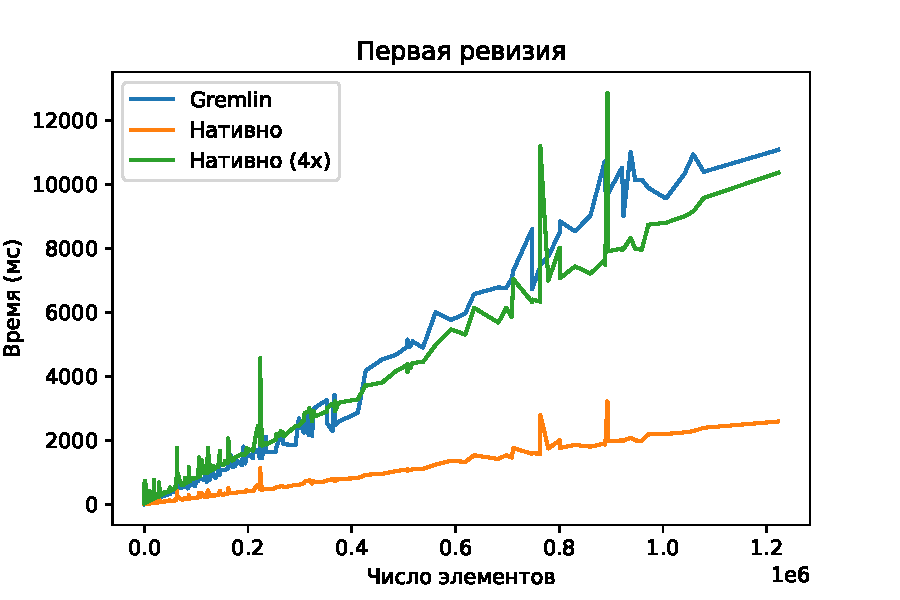
\includegraphics{img/ecr-plot.pdf}
\end{figure}

\begin{figure}[!h]
\caption{График зависимости времени исполнения запроса от числа элементов для запроса <<Список файлов ревизии>>}\label{fig-rec}
\centering
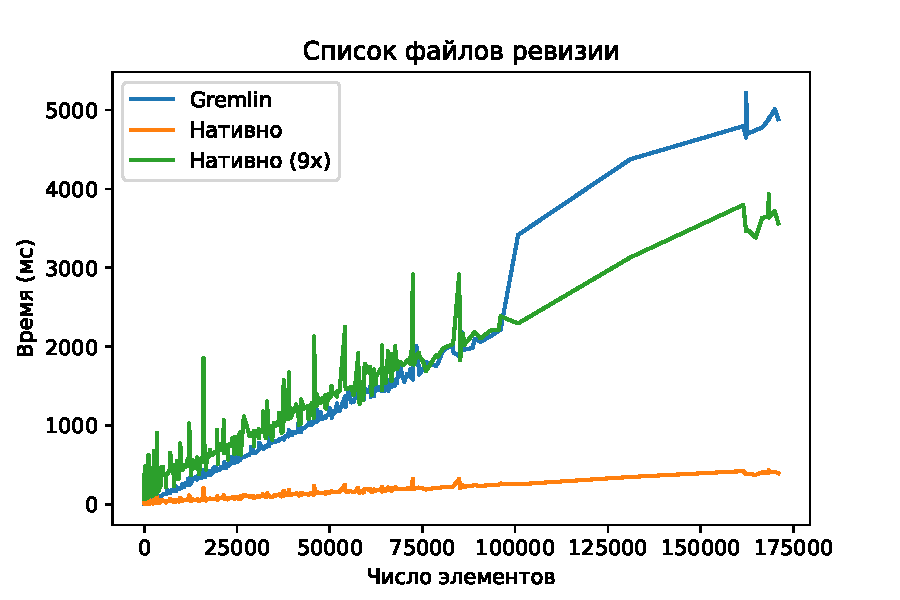
\includegraphics{img/rec-plot.pdf}
\end{figure}

\begin{figure}[!h]
\caption{График зависимости времени исполнения запроса от числа элементов для запроса <<Дерево ревизий снимка>>}\label{fig-snp}
\centering
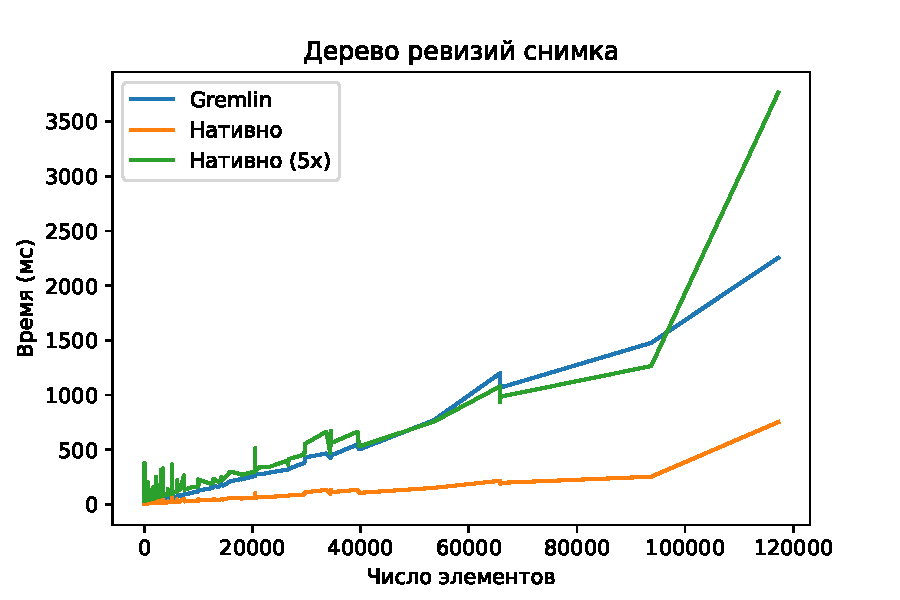
\includegraphics{img/snp-plot.pdf}
\end{figure}

Из графиков для первого и третьего запросов следует, что Gremlin запросы испытывают замедление в 4--5 раз по сравнению с нативным.
При этом на графике для второго запроса видно, что замедление составляет 9 раз. Причиной такой разницы вероятно является тот факт, что первый и третий запросы являются алгоритмическим аналогом своих нативных версий. Второй же запрос с точки зрения заложенного алгоритма несколько отличается от нативной реализации. Проблема заключается в том, что наиболее оптимальным методом для данного запроса является поиск с возвратом (англ. backtracking). Именно этот подход был реализован в нативной версии, однако изученные мной Gremlin шаги не позволяют осуществить этот подход. Из-за этого в Gremlin реализации приходится работать с каждым путем от начальной вершины до конечной отдельно. Если изменить нативную реализацию так, чтобы она отражала Gremlin реализацию, то в результатах можно увидеть такое же замедление в 4--5 раз, как и на других запросах. График для обновленного запроса представлен на рисунке~\ref{fig-rec2}.

\begin{figure}[!h]
\caption{График зависимости времени исполнения запроса от числа элементов для запроса <<Список файлов ревизии>>}\label{fig-rec2}
\centering
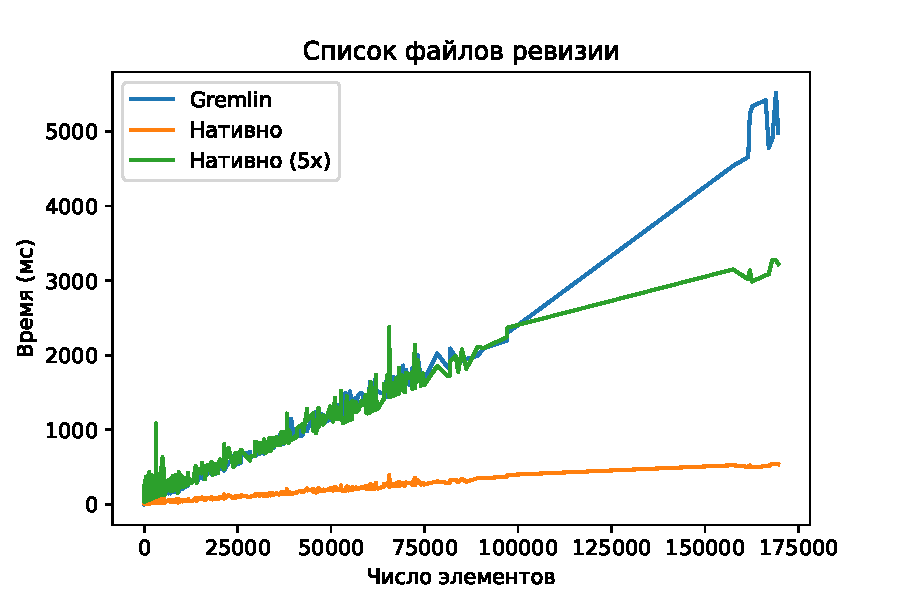
\includegraphics{img/rec2-plot.pdf}
\end{figure}

Из этого можно заключить, что привязка Gremlin к TinkerPop замедляет исполнение запроса в 4--5 раз. При этом важно сформулировать запрос оптимально, что для некоторых специфических случаев не всегда возможно.

\section{Тестирование на других графах}

Чтобы убедиться в том, что полученные результаты тестирования не специфичны для выбранного графа, а универсальны, тесты также были проведены и на нескольких других графах. В интересах полноты тестирования следовало выбрать максимально <<отличающиеся>> графы. В качестве меры отличия была выбрана средняя степень вершины. Выбрав максимально отличающиеся по средней степени вершины графы, под тестирование попадут графы с весьма разной структурой, что поможет сделать выводы об универсальности полученных ранее результатов.

В качестве тестируемых графов были выбраны два дополнительных набора данных, доступных на странице WebGraph~\cite{webgraph-datasets}, а именно \texttt{hollywood-2011} и \texttt{imdb-2021}. Среди представленных наборов данных эти наборы максимально отличаются от \texttt{python3k} по средней степени вершины: 105,0 у \texttt{hollywood-2011} и 3,58 у \texttt{imdb-2021}, вместо 26,7 у \texttt{python3k}. Формулировка и реализация доменно-специфических запросов на этих графах потребовала бы много времени, поэтому было решено определить один запрос общий для всех трех графов. В качестве такого запроса был выбран обход в глубину. Такой запрос обходит весь граф и не зависит от его свойств. Реализация запроса на Gremlin представлена на листинге~\ref{lst:gremlin-dfs}.

\begin{lstlisting}[float=!h,caption={Запрос, обходящий весь граф},label={lst:gremlin-dfs}]
g.V().not(in())
 .repeat(out().dedup())
\end{lstlisting}

Проведенный анализ времени работы подтвердил полученные ранее результаты: замедление исполнения запроса в 4--5 раз по сравнению с нативной реализацией. Объем дополнительно затрачиваемой памяти сравним с размером помеченного графа в памяти, что означает двукратное ухудшение. При этом стоит отметить, что подобный запрос даже в нативном виде не является осуществимым на больших графах, так как обходит и сохраняет все вершины, поэтому в реальных случаях ухудшение в использовании памяти будет меньше.
\chapterconclusion

В этой главе был описан метод проведения тестирования результатов. Был выбран набор данных, сформулированы запросы, и проведен анализ эффективности их исполнения, показывающий, что получая возможность исполнять Gremlin запросы в своей системе, пользователь столкнется с 4--5 кратным замедлением их исполнения.

\startconclusionpage

В данной работе была описана разработанная библиотека, связывающая фреймворки WebGraph и TinkerPop, и позволяющая осуществлять немодифицирующие Gremlin запросы к любым графам, сжатым фреймворком WebGraph. Это позволяет использовать высокоуровневый доменно-ориентированный язык для формулировки запросов к графу, при этом сохраняя возможность пользоваться эффективностью WebGraph.

Были реализованы интерфейсы Apache TinkerPop, что позволило наладить взаимодействие между Gremlin и WebGraph. Также была добавлена поддержка свойств вершин и ребер, позволяющая формулировать широкий набор запросов. Реализация стандартных подходов к работе со свойствами в WebGraph, реализация исполнителя как строковых Gremlin запросов, так и сформулированных с использованием Gremlin-Java DSL, а также распространение проекта в виде Maven-зависимости позволяет с минимальной настройкой начать пользоваться библиотекой в своей системе.

Эта возможность была использована командой Software Heritage. В рамках работы была реализована поддержка графа репозиториев Software Heritage, и добавлена в репозиторий проекта.

Согласно проведенному тестированию было выявлено, что эффективность исполнения Gremlin запросов по сравнению с нативной реализацией снижается в 4--5 раз. При этом разработанная библиотека впервые позволяет запускать Gremlin запросы на крупных графах на относительно недорогом компьютере.

Дальнейшее развитие проекта возможно в первую очередь в области оптимизаций связки фреймворков. Реализация ряда эвристик может снизить потерю в эффективности, тем самым сделав библиотеку еще более применимой на практике.

\printmainbibliography

\end{document}
